% Lezione del 14/04/2021

\documentclass[../main.tex]{subfiles}

\begin{document}

\chapter{Chiamata di funzione}
La chiamata di funzione, in MIPS, è costituita da 2 parti:
\begin{itemize}
    \item \textbf{caller}: funzione chiamante
    \begin{itemize}
        \item passa gli argomenti alla funzione chiamata
        \item effettua un salto alla funzione chiamata*
    \end{itemize}
    \item \textbf{callee}: funzione chiamata
    \begin{itemize}
        \item legge i parametri (corrispondono agli argomenti passati)
        \item esegue le istruzioni che appartengono alla funzione
        \item può restituire un risultato al chiamante
        \item deve ritornare al punto di chiamata (indirizzo di
        ritorno\footnote{Indirizzo di ritorno: è l'indirizzo a cui
        torna la funzione dopo che è stata eseguita.})
        \item il codice delle funzioni non deve sovrascrivere registri
        o memoria che sono utilizzati dal chiamante
    \end{itemize}
\end{itemize}

\vspace*{2mm}

\noindent
*\textbf{Nota bene}: l'operazione di salto è un'operazione in cui la
CPU:
\begin{itemize}
    \item cambia il valore del Program Counter
    \item salva il valore di ritorno
\end{itemize}

\noindent
\begin{table}[h!]
    \begin{minipage}{.02\linewidth}
        \hspace*{0cm}
    \end{minipage}
    \begin{minipage}{.2\linewidth}
        \section*{Esempio}
    \end{minipage}
    \begin{minipage}{.5\linewidth}
        \textbf{Codice C} \\
        \texttt{
            void main() \{ \\
            \hspace*{0cm} \hspace*{0cm} \hspace*{0cm} \hspace*{0cm} int y; \\
            \hspace*{0cm} \hspace*{0cm} \hspace*{0cm} \hspace*{0cm} y = sum(42, 7); \\
            \hspace*{0cm} \hspace*{0cm} \hspace*{0cm} \hspace*{0cm} \dots \\
            \} \\
            \\
            int sum(int a, int b) \{ \\
            \hspace*{0cm} \hspace*{0cm} \hspace*{0cm} \hspace*{0cm} return (a + b); \\
            \} \\
        }
    \end{minipage}
\end{table}

\section{Funzione chiamante e chiamata}
Gestione delle operazioni svolte tra funzione chiamante e chiamata:
\begin{itemize}
    \item la chiamata della funzione viene gestita dall'istruzione \texttt{jump and link} (\texttt{jal})
    \item l'operazione di ritorno, che mi fa tornare al chiamante,
    è fatta attraverso l'istruzione \texttt{jump register} (\texttt{jr})
    \item il passaggio degli argomenti avviene utilizzando i registri da
    \texttt{\$a0} a \texttt{\$a3} (4 registri)
    \item il valore di ritorno è contenuto nel registro \texttt{\$v0}
\end{itemize}

\vspace*{2mm}

\noindent
\underline{\textbf{Nota bene}: se la funzione ha più di 4 argomenti allora sono
obbligato ad utilizzare lo stack} \\
\underline{(più lento in quanto utilizza la RAM).}

\newpage

\subsection{Jump and Link}
L'istruzione \texttt{Jump and link} (\texttt{jal}) è di tipo J. \\[3mm]
\textbf{Esempio}
\vspace*{-2mm}
\begin{table}[h!]
    \texttt{jal proc} \\[2mm]
    \setlength{\tabcolsep}{0pt}
    \begin{tabular}{ c c c | c c | c }
        \vspace*{-4.2mm} & \multicolumn{2}{ p{(\linewidth / 48) * 6} }{} & \multicolumn{2}{ p{((\linewidth / 48) * 26)} }{} \\
        \cline{2-5}
        \multicolumn{1}{ c | }{} & \multicolumn{2}{ c | }{\texttt{op}} & \multicolumn{2}{ c | }{\texttt{addr}} & \\
        \cline{2-5}
        \rule{0pt}{.8\normalbaselineskip} & \multicolumn{1}{ l }{31} & \multicolumn{1}{ r }{26\hspace*{.5mm}} & \multicolumn{1}{ l }{\hspace*{.5mm}25} & \multicolumn{1}{ r }{0} & \\
    \end{tabular}
\end{table}

\noindent
Esegue le seguenti operazioni:
\begin{itemize}
    \item modifica il valore del Program Counter
    per saltare all'indirizzo della procedura \texttt{proc}
    \item il chiamante scrive l'indirizzo di ritorno nel registro
    \texttt{\$ra} (\textit{return address} register)
\end{itemize}

\vspace*{2mm}

\noindent
\underline{\textbf{Nota bene}: non è una pseudoistruzione in quanto la CPU esegue
2 operazioni ma a livello di codice} \\
\underline{equivale ad un'unica istruzione.}

\subsection*{Esempio}
\begin{tabular}{ p{8cm} p{8cm} }
    \textbf{Codice C} & \textbf{Codice MIPS assembly} \\
    \texttt{int main() \{} \\
    \texttt{\hspace*{0cm} \hspace*{0cm} \hspace*{0cm} \hspace*{0cm} simple();} & \texttt{{\color{black} \textbf{0x00400200}} main: jal simple} \\
    \texttt{\hspace*{0cm} \hspace*{0cm} \hspace*{0cm} \hspace*{0cm} a = b + c;} & \texttt{{\color{red} \textbf{0x00400204}} add \$s0, \$s1, \$s2} \\
    \texttt{\}} & \texttt{\dots} \\
    \\
    \texttt{void simple() \{} \\
    \texttt{\hspace*{0cm} \hspace*{0cm} \hspace*{0cm} \hspace*{0cm} return;} & \texttt{{\color{blue} \textbf{0x00401020}} simple: jr \$ra} \\
    \texttt{\}} \\
\end{tabular}

\vspace*{5mm}

\noindent
\begin{tabular}{ l l }
    \textbf{\texttt{jal}:} & Salva l'indirizzo di ritorno (\texttt{\$ra = PC + 4 = {\color{red} \textbf{0x00400204}}}) \\
    & Salta alla label \texttt{simple} (\texttt{{\color{blue} \textbf{0x00401020}}}) \\
    \textbf{\texttt{jr \$ra}:} & Salta all'indirizzo salvato nel registro \texttt{\$ra} (\texttt{{\color{red} \textbf{0x00400204}}}) \\
\end{tabular}

\vspace*{1cm}

\section*{Esempio}
Nella convenzione MIPS:
\begin{itemize}
    \item gli argomenti vengono salvati nei registri
          da \texttt{\$a0} a \texttt{\$a3}
    \item il valore di ritorno nel registro \texttt{\$v0}
\end{itemize}
\begin{table}[h!]
    \centering

    \begin{tabular}{ l l }
        \textbf{Codice C} & \textbf{Codice MIPS assembly} \\
        & \texttt{\# \$s0 = y} \\
        \texttt{int main() \{} & \texttt{main:} \\
        \texttt{\hspace*{0cm} \hspace*{0cm} \hspace*{0cm} \hspace*{0cm} int y;} & \texttt{\hspace*{0cm} \hspace*{0cm} \hspace*{0cm} \hspace*{0cm} \dots} \\
        \texttt{\hspace*{0cm} \hspace*{0cm} \hspace*{0cm} \hspace*{0cm} \dots} & \texttt{\hspace*{0cm} \hspace*{0cm} \hspace*{0cm} \hspace*{0cm} addi \$a0, \$0, 2 \hspace*{0cm} \hspace*{0cm} \hspace*{0cm} \# argument 0 = 2} \\
        \texttt{\hspace*{0cm} \hspace*{0cm} \hspace*{0cm} \hspace*{0cm} y = diffofsums(2, 3, 4, 5); // 4 arguments} & \texttt{\hspace*{0cm} \hspace*{0cm} \hspace*{0cm} \hspace*{0cm} addi \$a1, \$0, 3 \hspace*{0cm} \hspace*{0cm} \hspace*{0cm} \# argument 1 = 3} \\
        \texttt{\hspace*{0cm} \hspace*{0cm} \hspace*{0cm} \hspace*{0cm} \dots} & \texttt{\hspace*{0cm} \hspace*{0cm} \hspace*{0cm} \hspace*{0cm} addi \$a2, \$0, 4 \hspace*{0cm} \hspace*{0cm} \hspace*{0cm} \# argument 2 = 4} \\
        \texttt{\}} & \texttt{\hspace*{0cm} \hspace*{0cm} \hspace*{0cm} \hspace*{0cm} addi \$a3, \$0, 5 \hspace*{0cm} \hspace*{0cm} \hspace*{0cm} \# argument 3 = 5} \\
        & \texttt{\hspace*{0cm} \hspace*{0cm} \hspace*{0cm} \hspace*{0cm} jal \hspace*{0cm} diffofsums \hspace*{0cm} \hspace*{0cm} \hspace*{0cm} \# call Function} \\
        & \texttt{\hspace*{0cm} \hspace*{0cm} \hspace*{0cm} \hspace*{0cm} add \hspace*{0cm} \$s0, \$v0, \$0 \hspace*{0cm} \# y = returned value} \\
        & \texttt{\hspace*{0cm} \hspace*{0cm} \hspace*{0cm} \hspace*{0cm} \dots} \\
        \\
        & \texttt{\# \$s0 = result} \\
        \texttt{int diffofsums(int f, int g, int h, int i) \{} & \texttt{diffofsums:} \\
        \texttt{\hspace*{0cm} \hspace*{0cm} \hspace*{0cm} \hspace*{0cm} int result;} & \texttt{\hspace*{0cm} \hspace*{0cm} \hspace*{0cm} \hspace*{0cm} add {\color{red} \textbf{\$t0}}, \$a0, \$a1 \hspace*{0cm} \# \$t0 = f + g} \\
        \texttt{\hspace*{0cm} \hspace*{0cm} \hspace*{0cm} \hspace*{0cm} result = (f + g) - (h + i);} & \texttt{\hspace*{0cm} \hspace*{0cm} \hspace*{0cm} \hspace*{0cm} add {\color{red} \textbf{\$t1}}, \$a2, \$a3 \hspace*{0cm} \# \$t1 = h + i} \\
        \texttt{\hspace*{0cm} \hspace*{0cm} \hspace*{0cm} \hspace*{0cm} return result; // return value} & \texttt{\hspace*{0cm} \hspace*{0cm} \hspace*{0cm} \hspace*{0cm} sub {\color{red} \textbf{\$s0}}, \$t0, \$t1 \hspace*{0cm} \# result = (f + g) - (h + i)} \\
        & \texttt{\hspace*{0cm} \hspace*{0cm} \hspace*{0cm} \hspace*{0cm} add \$v0, \$s0, \$0 \hspace*{0cm} \hspace*{0cm} \# put return value in \$v0} \\
        & \texttt{\hspace*{0cm} \hspace*{0cm} \hspace*{0cm} \hspace*{0cm} jr \$ra \hspace*{0cm} \hspace*{0cm} \hspace*{0cm} \hspace*{0cm} \hspace*{0cm} \hspace*{0cm} \hspace*{0cm} \hspace*{0cm} \hspace*{0cm} \hspace*{0cm} \hspace*{0cm} \hspace*{0cm} \# return to caller} \\
        \texttt{\}} & \\
    \end{tabular}
\end{table}

\noindent
La \texttt{diffofsums}:
\begin{itemize}
    \item sovrascrive 3 registri: \texttt{\$t0}, \texttt{\$t1}, \texttt{\$s0}
    \item può usare lo stack per salvare
    temporaneamente questi registri
\end{itemize}

\newpage

\section{Stack}
Lo Stack è una struttura dati di tipo Last-In First-Out (LIFO) e
si basa sulla presenza di un registro, lo \textbf{Stack Pointer},
\underline{che punta all'ultimo valore inserito}. \\[2mm]
Esistono due tipi di operazioni che fanno accesso allo Stack:
\begin{itemize}
    \item push operazione che scrive dallo Stack
    \item pop operazione che legge dallo Stack
\end{itemize}

\vspace{2mm}

\noindent
Nell'architettura MIPS, lo Stack Pointer cresce per numero di indirizzi
descescente.

\begin{table}[htb!]
    \begin{minipage}{.45\linewidth}
        \renewcommand{\arraystretch}{1.2}
        \setlength{\tabcolsep}{18pt}
        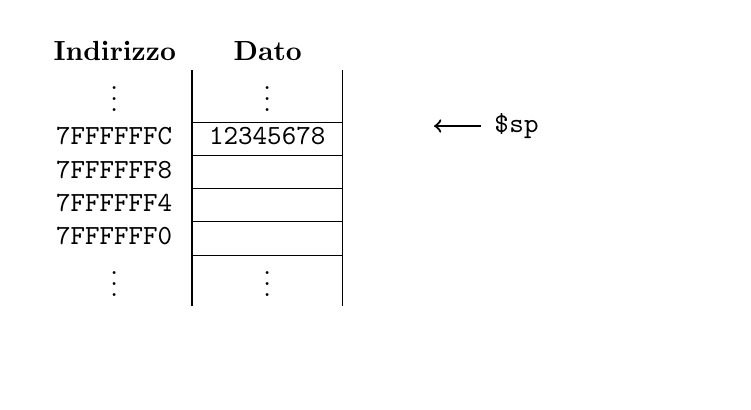
\begin{tikzpicture}
            \node(table) {
                \begin{tabular}{ c | c | }
                    \multicolumn{1}{c}{\textbf{Indirizzo}} & \multicolumn{1}{c}{\textbf{Dato}} \\
                    \vdots & \vdots \\
                    \cline{2-2}
                    \texttt{7FFFFFFC} & \texttt{12345678} \\
                    \cline{2-2}
                    \texttt{7FFFFFF8} & \\
                    \cline{2-2}
                    \texttt{7FFFFFF4} & \\
                    \cline{2-2}
                    \texttt{7FFFFFF0} & \\
                    \cline{2-2}
                    \vdots & \vdots \\
                    \multicolumn{2}{c}{} \\
                    \multicolumn{2}{c}{} \\
                \end{tabular}
            };
    
            \draw [<-, thick]
                (3.1,1) -- (3.7,1);
    
            \node[text width=5cm, align=center] at (4.15,1) {\texttt{\$sp}};
    
        \end{tikzpicture}
    \end{minipage}
    \begin{minipage}{.02\linewidth}
        \hspace*{0cm}
    \end{minipage}
    \begin{minipage}{.45\linewidth}
        \setlength{\tabcolsep}{18pt}
        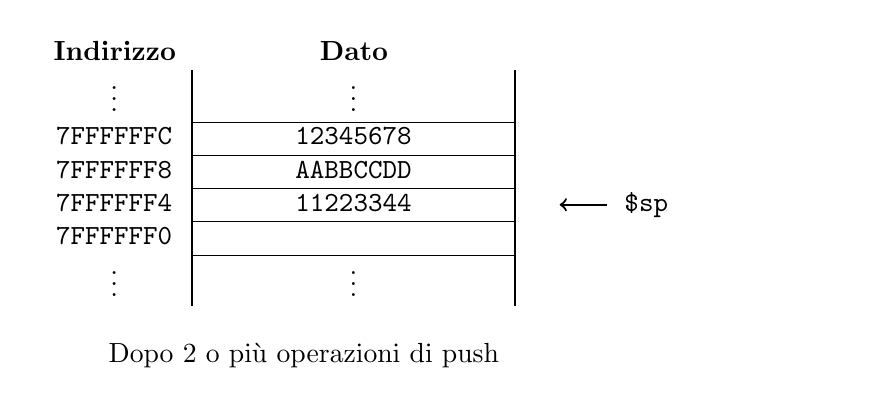
\begin{tikzpicture}
            \node(table) {
                \begin{tabular}{ c | c | }
                    \multicolumn{1}{c}{\textbf{Indirizzo}} & \multicolumn{1}{c}{\textbf{Dato}} \\
                    \vdots & \vdots \\
                    \cline{2-2}
                    \texttt{7FFFFFFC} & \texttt{12345678} \\
                    \cline{2-2}
                    \texttt{7FFFFFF8} & \texttt{AABBCCDD} \\
                    \cline{2-2}
                    \texttt{7FFFFFF4} & \texttt{11223344} \\
                    \cline{2-2}
                    \texttt{7FFFFFF0} & \\
                    \cline{2-2}
                    \vdots & \vdots \\
                    \multicolumn{2}{c}{} \\
                    \multicolumn{2}{c}{\hspace*{7mm}Dopo 2 o più operazioni di push} \\
                \end{tabular}
            };
    
            \draw [<-, thick]
                (3.6,0) -- (4.2,0);
    
            \node[text width=5cm, align=center] at (4.7,0) {\texttt{\$sp}};
    
        \end{tikzpicture}
    \end{minipage}
\end{table}

\noindent
Lo Stack diventa necessario quando si presenta il problema di
sovrascrittura nei registri; in questo caso, lo stack riesce a
salvaguardare il contenuto di questi registri. \\[5mm]
\textbf{Esempio} \\
\texttt{diffofsums} sovrascrive 3 registri: \texttt{\$t0}, \texttt{\$t1}, \texttt{\$s0} \\[2mm]
\textbf{Codice MIPS assembly} \\
\texttt{
    \# \$s0 = result \\
    diffofsums: \\
    \hspace*{0cm} \hspace*{0cm} \hspace*{0cm} \hspace*{0cm} add {\color{red} \textbf{\$t0}}, \$a0, \$a1 \hspace*{0cm} \# \$t0 = f + g \\
    \hspace*{0cm} \hspace*{0cm} \hspace*{0cm} \hspace*{0cm} add {\color{red} \textbf{\$t1}}, \$a2, \$a3 \hspace*{0cm} \# \$t1 = h + i \\
    \hspace*{0cm} \hspace*{0cm} \hspace*{0cm} \hspace*{0cm} sub {\color{red} \textbf{\$s0}}, \$t0, \$t1 \hspace*{0cm} \# result = (f + g) - (h + i) \\
    \hspace*{0cm} \hspace*{0cm} \hspace*{0cm} \hspace*{0cm} add \$v0, \$s0, \$0 \hspace*{0cm} \hspace*{0cm} \# put return value in \$v0 \\
    \hspace*{0cm} \hspace*{0cm} \hspace*{0cm} \hspace*{0cm} jr \$ra \hspace*{0cm} \hspace*{0cm} \hspace*{0cm} \hspace*{0cm} \hspace*{0cm} \hspace*{0cm} \hspace*{0cm} \hspace*{0cm} \hspace*{0cm} \hspace*{0cm} \hspace*{0cm} \hspace*{0cm} \# return to caller \\
}

\newpage

\subsection{Stack Frame}
Lo Stack Frame:
\begin{itemize}
    \item è l'area dello Stack che utilizza una funzione nel
    momento in cui viene eseguita
    \item viene predisposto, per certi versi al chiamante
    e per certi versi alla funzione chiamata
    \item può essere creato dalla funzione chiamante se ho
    bisogno di più di 4 parametri
\end{itemize}

\subsection*{Esempio}
\texttt{\# \$s0 = result \\
    diffofsums: \\
    \textbf{\hspace*{0cm} \hspace*{0cm} \hspace*{0cm} \hspace*{0cm} addi \$sp, \$sp, -12 \hspace*{0cm} \# crea lo spazio nello stack per salvare i 3 registri} \\
    \textbf{\hspace*{0cm} \hspace*{0cm} \hspace*{0cm} \hspace*{0cm} sw \$s0, 8(\$sp) \hspace*{0cm} \hspace*{0cm} \hspace*{0cm} \hspace*{0cm} \hspace*{0cm} \# scrive \$s0 nello stack} \\
    \textbf{\hspace*{0cm} \hspace*{0cm} \hspace*{0cm} \hspace*{0cm} sw \$t0, 4(\$sp) \hspace*{0cm} \hspace*{0cm} \hspace*{0cm} \hspace*{0cm} \hspace*{0cm} \# scrive \$t0 nello stack} \\
    \textbf{\hspace*{0cm} \hspace*{0cm} \hspace*{0cm} \hspace*{0cm} sw \$t1, 0(\$sp) \hspace*{0cm} \hspace*{0cm} \hspace*{0cm} \hspace*{0cm} \hspace*{0cm} \# scrive \$t1 nello stack} \\
    \hspace*{0cm} \hspace*{0cm} \hspace*{0cm} \hspace*{0cm} add \$t0, \$a0, \$a1 \hspace*{0cm} \hspace*{0cm} \# \$t0 = f + g \\
    \hspace*{0cm} \hspace*{0cm} \hspace*{0cm} \hspace*{0cm} add \$t1, \$a2, \$a3 \hspace*{0cm} \hspace*{0cm} \# \$t1 = h + i \\
    \hspace*{0cm} \hspace*{0cm} \hspace*{0cm} \hspace*{0cm} sub \$s0, \$t0, \$t1 \hspace*{0cm} \hspace*{0cm} \# risultato = (f + g) - (h + i) \\
    \hspace*{0cm} \hspace*{0cm} \hspace*{0cm} \hspace*{0cm} add \$v0, \$s0, \$0 \hspace*{0cm} \hspace*{0cm} \hspace*{0cm} \# inserisce il valore di ritorno nel registro \$v0 \\
    \textbf{\hspace*{0cm} \hspace*{0cm} \hspace*{0cm} \hspace*{0cm} lw \$t1, 0(\$sp) \hspace*{0cm} \hspace*{0cm} \hspace*{0cm} \hspace*{0cm} \hspace*{0cm} \# ripristina \$t1 dallo stack} \\
    \textbf{\hspace*{0cm} \hspace*{0cm} \hspace*{0cm} \hspace*{0cm} lw \$t0, 4(\$sp) \hspace*{0cm} \hspace*{0cm} \hspace*{0cm} \hspace*{0cm} \hspace*{0cm} \# ripristina \$t0 dallo stack} \\
    \textbf{\hspace*{0cm} \hspace*{0cm} \hspace*{0cm} \hspace*{0cm} lw \$s0, 8(\$sp) \hspace*{0cm} \hspace*{0cm} \hspace*{0cm} \hspace*{0cm} \hspace*{0cm} \# ripristina \$s0 dallo stack} \\
    \textbf{\hspace*{0cm} \hspace*{0cm} \hspace*{0cm} \hspace*{0cm} addi \$sp, \$sp, 12 \hspace*{0cm} \hspace*{0cm} \# dealloca lo spazio nello stack} \\
    \hspace*{0cm} \hspace*{0cm} \hspace*{0cm} \hspace*{0cm} jr \$ra \hspace*{0cm} \hspace*{0cm} \hspace*{0cm} \hspace*{0cm} \hspace*{0cm} \hspace*{0cm} \hspace*{0cm} \hspace*{0cm} \hspace*{0cm} \hspace*{0cm} \hspace*{0cm} \hspace*{0cm} \hspace*{0cm} \# ritorna al chiamante \\
}

\begin{table}[h!]
    \begin{minipage}{.33\linewidth}
        \begin{tikzpicture}
            \node(table) {
                \renewcommand{\arraystretch}{1.2}
                \setlength{\dashlinegap}{2pt}
                \setlength{\tabcolsep}{12pt}
                \begin{tabular}{ c | >{\centering\arraybackslash}p{1cm} | }
                    \multicolumn{1}{c}{\textbf{Indirizzo}} & \multicolumn{1}{c}{\textbf{Dato}} \\
                    \multicolumn{1}{ c : }{\vdots} & \multicolumn{1}{ c : }{\vdots} \\
                    \cline{2-2}
                    \texttt{FC} & \texttt{?} \\
                    \cline{2-2}
                    \texttt{F8} & \\
                    \cline{2-2}
                    \texttt{F4} & \\
                    \cline{2-2}
                    \texttt{F0} & \\
                    \cline{2-2}
                    \multicolumn{1}{ c : }{\vdots} & \multicolumn{1}{ c : }{\vdots} \\
                    \multicolumn{2}{l}{\textbf{(a)}} \\
                    \multicolumn{2}{c}{} \\
                    \multicolumn{2}{c}{\makecell{Prima della \\ \texttt{diffofsum}}} \\
                \end{tabular}
            };
    
            \draw [<-, thick]
                (2.4,1.4) -- (2.9,1.4);
    
            \node[text width=5cm, align=center] at (3.35,1.4) {\texttt{\$sp}};
    
        \end{tikzpicture}
    \end{minipage}
    \begin{minipage}{.33\linewidth}
        \begin{tikzpicture}
            \node(table) {
                \renewcommand{\arraystretch}{1.2}
                \setlength{\dashlinegap}{2pt}
                \setlength{\tabcolsep}{12pt}
                \begin{tabular}{ c | >{\centering\arraybackslash}p{1cm} | }
                    \multicolumn{1}{c}{\textbf{Indirizzo}} & \multicolumn{1}{c}{\textbf{Dato}} \\
                    \multicolumn{1}{ c : }{\vdots} & \multicolumn{1}{ c : }{\vdots} \\
                    \cline{2-2}
                    \texttt{FC} & \texttt{?} \\
                    \cline{2-2}
                    \texttt{F8} & \texttt{\$s0} \\
                    \cline{2-2}
                    \texttt{F4} & \texttt{\$t0} \\
                    \cline{2-2}
                    \texttt{F0} & \texttt{\$t1} \\
                    \cline{2-2}
                    \multicolumn{1}{ c : }{\vdots} & \multicolumn{1}{ c : }{\vdots} \\
                    \multicolumn{2}{l}{\textbf{(b)}} \\
                    \multicolumn{2}{c}{} \\
                    \multicolumn{2}{c}{\makecell{Durante la \\ \texttt{diffofsum}}} \\
                \end{tabular}
            };
    
            \draw [<-, thick]
                (2.4,-.1) -- (2.9,-.1);
            \node[text width=5cm, align=center] at (3.35,-.1) {\texttt{\$sp}};
            
            \draw (-.9,1.175) -- (-1.1,1.175) -- (-1.1,-.35) -- (-.9,-.35);
            \node[text width=5cm, align=center, rotate=90] at (-1.35,.4) {\small stack frame};
    
        \end{tikzpicture}
    \end{minipage}
    \begin{minipage}{.33\linewidth}
        \begin{tikzpicture}
            \node(table) {
                \renewcommand{\arraystretch}{1.2}
                \setlength{\dashlinegap}{2pt}
                \setlength{\tabcolsep}{12pt}
                \begin{tabular}{ c | >{\centering\arraybackslash}p{1cm} | }
                    \multicolumn{1}{c}{\textbf{Indirizzo}} & \multicolumn{1}{c}{\textbf{Dato}} \\
                    \multicolumn{1}{ c : }{\vdots} & \multicolumn{1}{ c : }{\vdots} \\
                    \cline{2-2}
                    \texttt{FC} & \texttt{?} \\
                    \cline{2-2}
                    \texttt{F8} & \\
                    \cline{2-2}
                    \texttt{F4} & \\
                    \cline{2-2}
                    \texttt{F0} & \\
                    \cline{2-2}
                    \multicolumn{1}{ c : }{\vdots} & \multicolumn{1}{ c : }{\vdots} \\
                    \multicolumn{2}{l}{\textbf{(c)}} \\
                    \multicolumn{2}{c}{} \\
                    \multicolumn{2}{c}{\makecell{Dopo la \\ \texttt{diffofsum}}} \\
                \end{tabular}
            };
    
            \draw [<-, thick]
                (2.4,1.4) -- (2.9,1.4);
    
            \node[text width=5cm, align=center] at (3.35,1.4) {\texttt{\$sp}};
    
        \end{tikzpicture}
    \end{minipage}
\end{table}

\end{document}